\chapter{Allgemeine Einführung}

Im weitesten Sinne kann man die Phonetik als die Wissenschaft der gesprochenen Sprache beschreiben. In der ersten Sitzung der Grundlagen-Vorlesung „Phonetik“ wurde eine Reihe differenzierter Definitionen präsentiert, bei denen vor allem die Sprachproduktion (\textit{Artikulation}), Transmission (\textit{Akustik}) und \textit{Perzeption} im Vordergrund stehen. Bei der Erforschung gesprochener Sprache kommen \textit{signalphonetische} und \textit{symbolphonetische} Untersuchungsansätze zur Anwendung. $\rightarrow$ {\tt L1\underline{\ }Einführung.pdf} 

Die \textit{Sprachkette} und das \textit{signalphonetische} Band (Abb.~\ref{fig1}) stellen die oben genannten Bereiche der Phonetik graphisch dar. Des Weiteren können in ihr die Neurophonetik, die sich mit der Sprechplanung und Sprachverarbeitung im Gehirn beschäftigt, sowie die Psycholinguistik, die unter anderem die menschliche Sprachfähigkeit untersucht, verortet werden.  Um den Bereich der Sprachtechnologie in der Sprachkette abzubilden müssen entweder der Sprecher (Sprachsynthese) und/oder der Hörer durch Computer   ausgetauscht werden. Das Prinzip der Sprachkette bleibt bestehen, aber die Komponenten müssen geändert bzw. ergänzt werden und Untersuchungsgegenstände ändern sich teilweise.

Während die P1-Vorlesung vorrangig Artikulation, Akustik und Perzeption und darüber hinaus die Phonologie, d.\thinspace h. die Lehre von den Funktionen von Lauten in einer Sprache, behandelt, werden in dieser Übung auch die anderen oben genannten Aspekte der Sprachkette beleuchtet und in einen phonetischen Gesamtrahmen eingebettet.

\begin{figure}[htbp]
\begin{center}
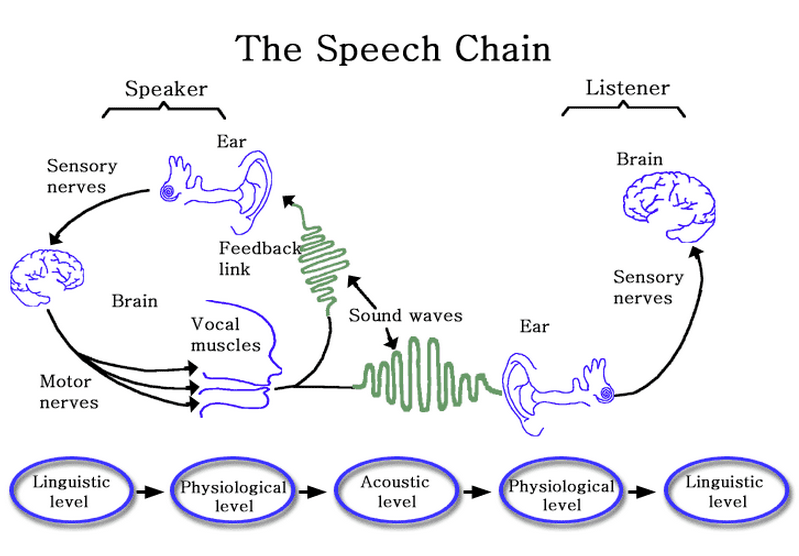
\includegraphics[width=\textwidth]{grafiken/allgemeine-einfuehrung/speech-chain.png}
\caption{nach Denes, P. B.; Pinson, E. N. (2012). The Speech Chain. The Physics And Biology Of Spoken Language.}
\label{fig1}
\end{center}
\end{figure}

\section{Stichworte zur ersten Stunde der Vorlesung} 

ABC-Prosodie,  Symbol- vs. Signalphonetik, Signalphonetisches Band, Sprachkette, Sprachlaut... $\rightarrow$ {\tt L1\underline{\ }Einführung.pdf} 


\section{Literatur}

Borden, G. J.; Harris, K. S., Raphael, L. J. (2011). \emph{Speech science primer. Physiology, acoustics, and perception of speech.} 6. Aufl. Baltimore: Lippincott Williams \& Wilkins. \newline\\
Bußmann, H. (2008). \emph{Lexikon der Sprachwissenschaft.} 4. Aufl. Stuttgart: Kröner. \newline\\
Clark, J. \& Yallop, C. (2007). \emph{An introduction to phonetics and phonology.} Malden u.\,a.:  Basil Blackwell.\newline\\
Gussenhoven, C. \& Jacobs, H. (2011). \emph{Understanding Phonology.} London  u.\,a.: Hodder.\newline\\
Hall, T. A. (2011).\emph{ Phonologie: Eine Einführung.} 2. Aufl. Berlin: Walter de Gruyter. \newline\\
International Phonetic Association (Hrsg.)(1999). \emph{Handbook of the International Phonetic Association}. Cambridge: Cambridge University Press. \newline\\
Kohler, K. J.(1995). \emph{Einführung in die Phonetik des Deutschen.} Berlin: Erich Schmidt. \newline\\
Ladefoged, P. (2003). \emph{Phonetic Data Analysis. An Introduction to Fieldwork and Instrumental Techniques}. Malden, MA u. a.: Blackwell.\newline\\
Ladefoged, P.; Johnson, K.  (2014). \emph{A course in phonetics.} 7.\,Aufl. Stamford u.\,a.: Cengage Learning. \newline\\
Ladefoged, P. \& Ferrari, S. (2012). \emph{Vowels and consonants.} An introduction to the sounds of language. 3.\,Aufl. Chichester: Wiley-Blackwell. \newline\\
Pompino-Marschall, B. (2009). \emph{Einführung in die Phonetik.} 3. Aufl. Berlin/New York: de Gruyter.  \newline\\
Reetz, H. (2003). \emph{Artikulatorische und akustische Phonetik.} 2.\,Aufl. Trier: Wissenschaftlicher Verlag.  \newline\\
Spencer, A. (1996). \emph{Phonology.} Oxford: Blackwell.\newline\\
Tillmann, H. G. \& Mansell, P. (1980). \emph{Phonetik: Lautsprachliche Zeichen, Sprachsignale und lautsprachlicher Kommunikationsprozeß.} Stuttgart: Klett-Cotta. \newline\\

\section{Interaktives Glossar}

Im Laufe des Semesters werden Ihnen einige Begriffe begegnen, über die Sie mehr wissen wollen oder mit denen Sie noch nicht soviel anfangen können. Hier haben Sie die Möglichkeit sich diese Wörter zu notieren und selbstständig, bzw. mit unserer Hilfe, Erklärungen zu finden. Glossare, Indexe oder Register finden sich in vielen der oben genannten Bücher; z.\,B. in Pompino-Marschall\,(2009), Reetz\,(2003), Draxler\,(2008) oder in Ladefoged \& Ferrari\,(2012). Bei Fragen stehen wir ihnen gerne zur Verfügung.  


